% !TEX root = ../main.tex
% --+ 20.10a Q2 +---------------------------------------------------------------
\begin{frame}{Uncorrected DIS Plots: $Q^2$}
    \label{20.10a::q2}

    \begin{figure}[t]
        \centering{
            \fbox{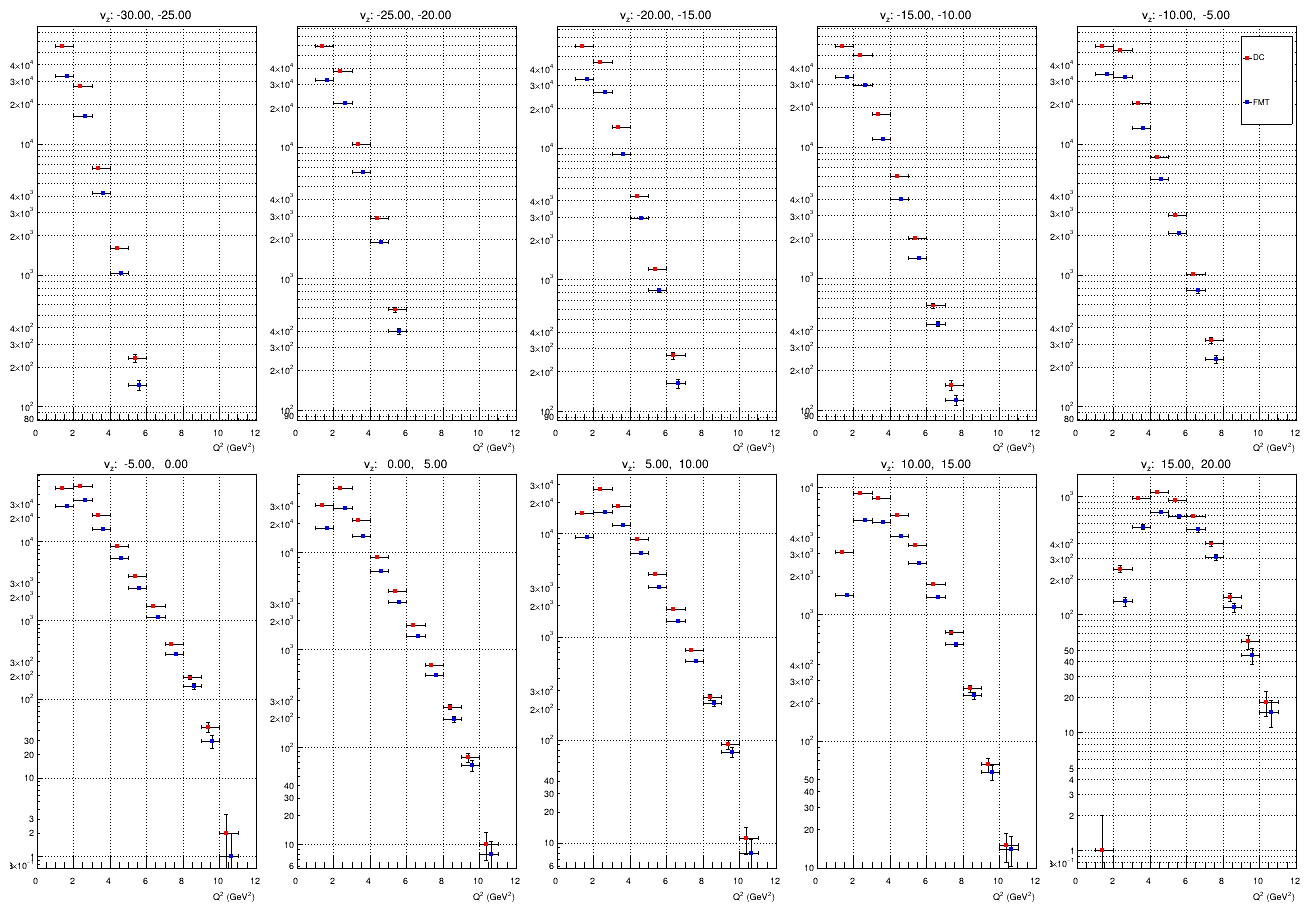
\includegraphics[width=0.72\textwidth]{10a_q2.png}}
        }
    \end{figure}

    \backref{12.12::q2}
\end{frame}

% --+ 20.10b NU +---------------------------------------------------------------
\begin{frame}{Uncorrected DIS Plots: $\nu$}
    \label{20.10b::nu}

    \begin{figure}[t]
        \centering{
            \fbox{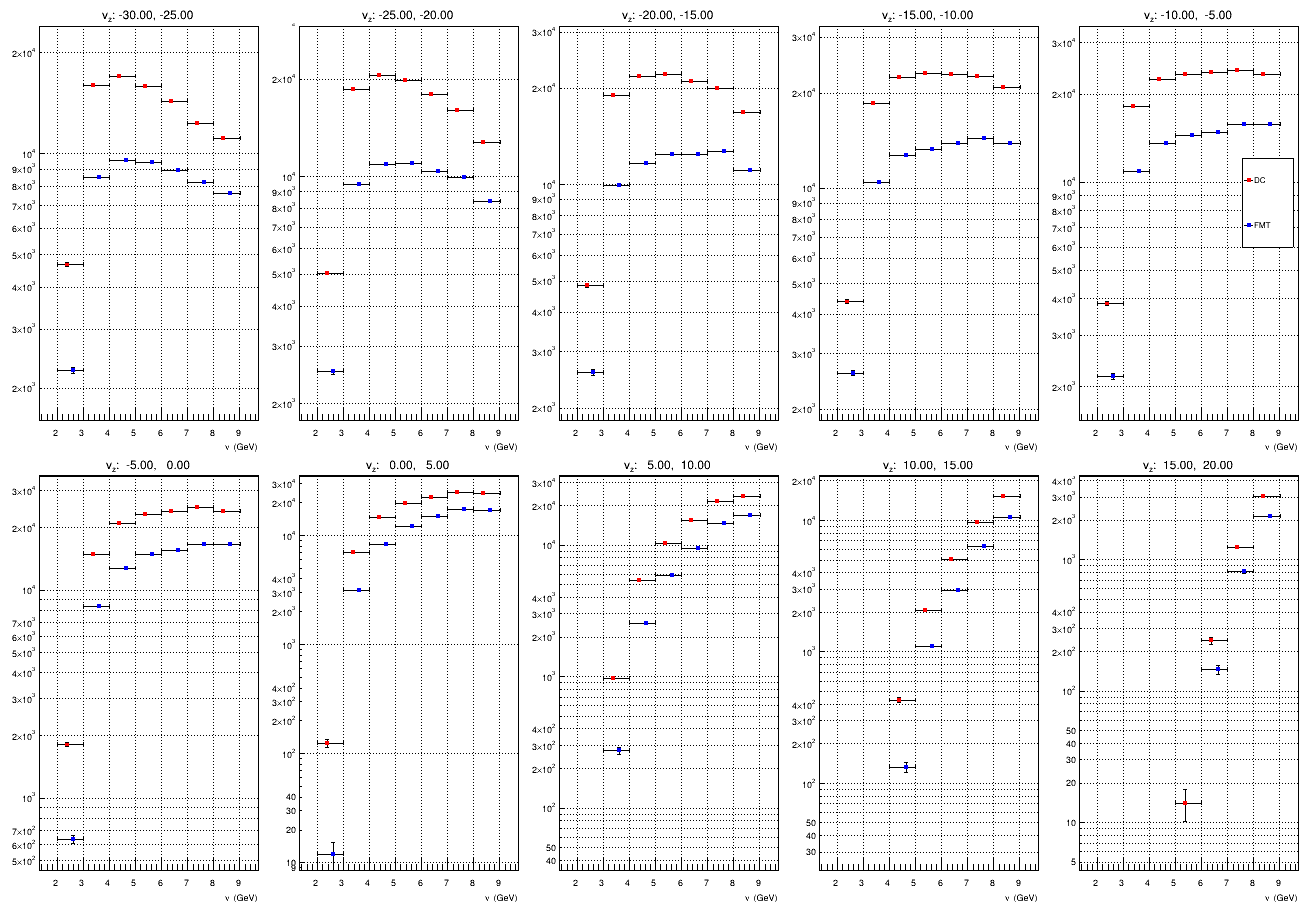
\includegraphics[width=0.72\textwidth]{10b_nu.png}}
        }
    \end{figure}

    \backref{12.13::nu}
\end{frame}

% --+ 20.10c zh pi+ +-----------------------------------------------------------
\begin{frame}{Uncorrected DIS Plots: $z_h$ for $\pi^+$}
    \label{20.10c::zh_pi+}

    \begin{figure}[t]
        \centering{
            \fbox{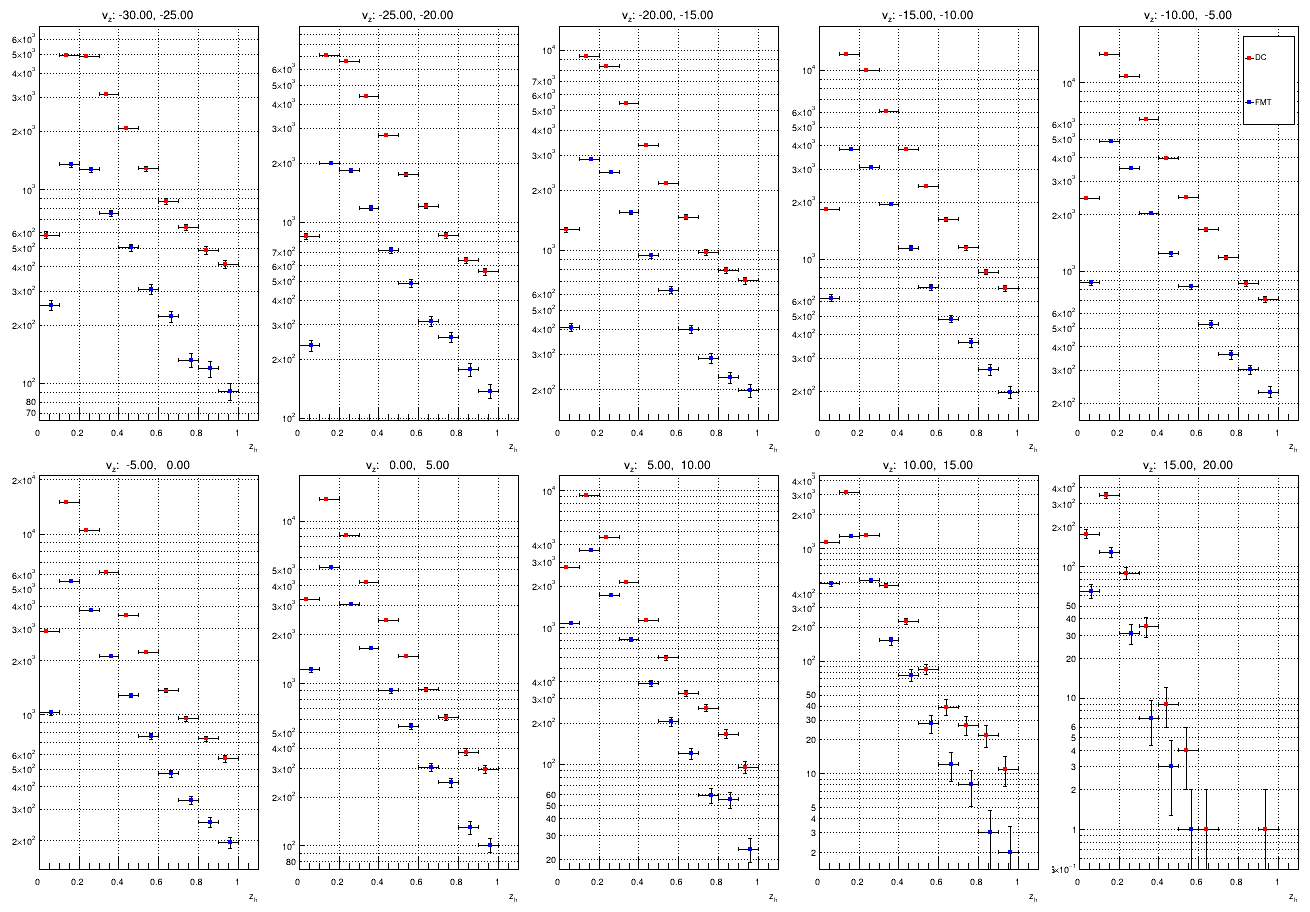
\includegraphics[width=0.72\textwidth]{10c_zh_pi+.png}}
        }
    \end{figure}

    \backref{12.14::zh}
\end{frame}

% --+ 20.10d zh pi- +-----------------------------------------------------------
\begin{frame}{Uncorrected DIS Plots: $z_h$ for $\pi^-$}
    \label{20.10d::zh_pi-}

    \begin{figure}[t]
        \centering{
            \fbox{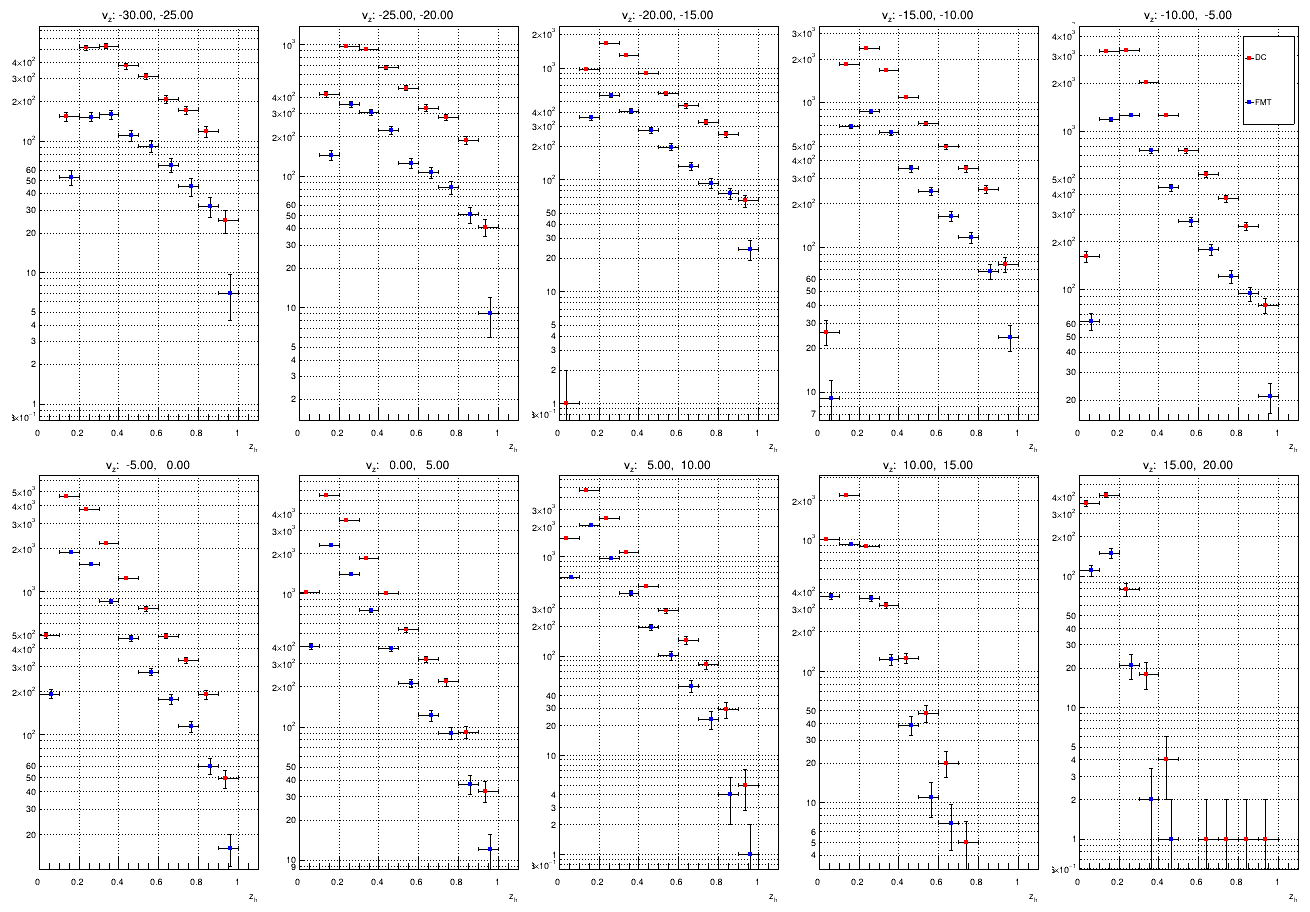
\includegraphics[width=0.72\textwidth]{10d_zh_pi-.png}}
        }
    \end{figure}

    \backref{12.14::zh}
\end{frame}

% --+ 20.10e pt2 pi+ +----------------------------------------------------------
\begin{frame}{Uncorrected DIS Plots: $p_T^2$ for $\pi^+$}
    \label{20.10e::pt2_pi+}

    \begin{figure}[t]
        \centering{
            \fbox{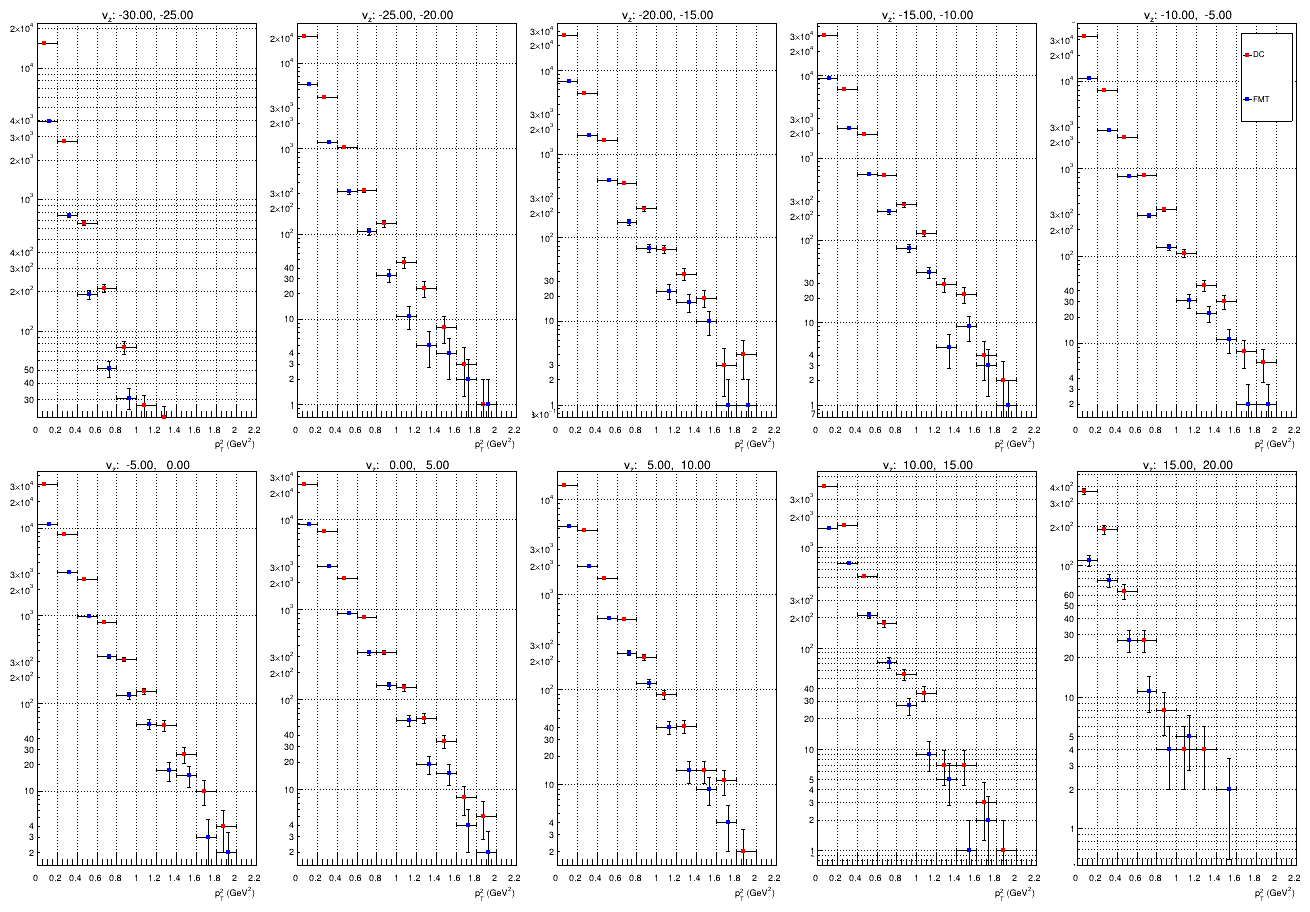
\includegraphics[width=0.72\textwidth]{10e_pt2_pi+.png}}
        }
    \end{figure}

    \backref{12.15::pt2}
\end{frame}

% --+ 20.10f pt2 pi- +----------------------------------------------------------
\begin{frame}{Uncorrected DIS Plots: $p_T^2$ for $\pi^-$}
    \label{20.10f::pt2_pi-}

    \begin{figure}[t]
        \centering{
            \fbox{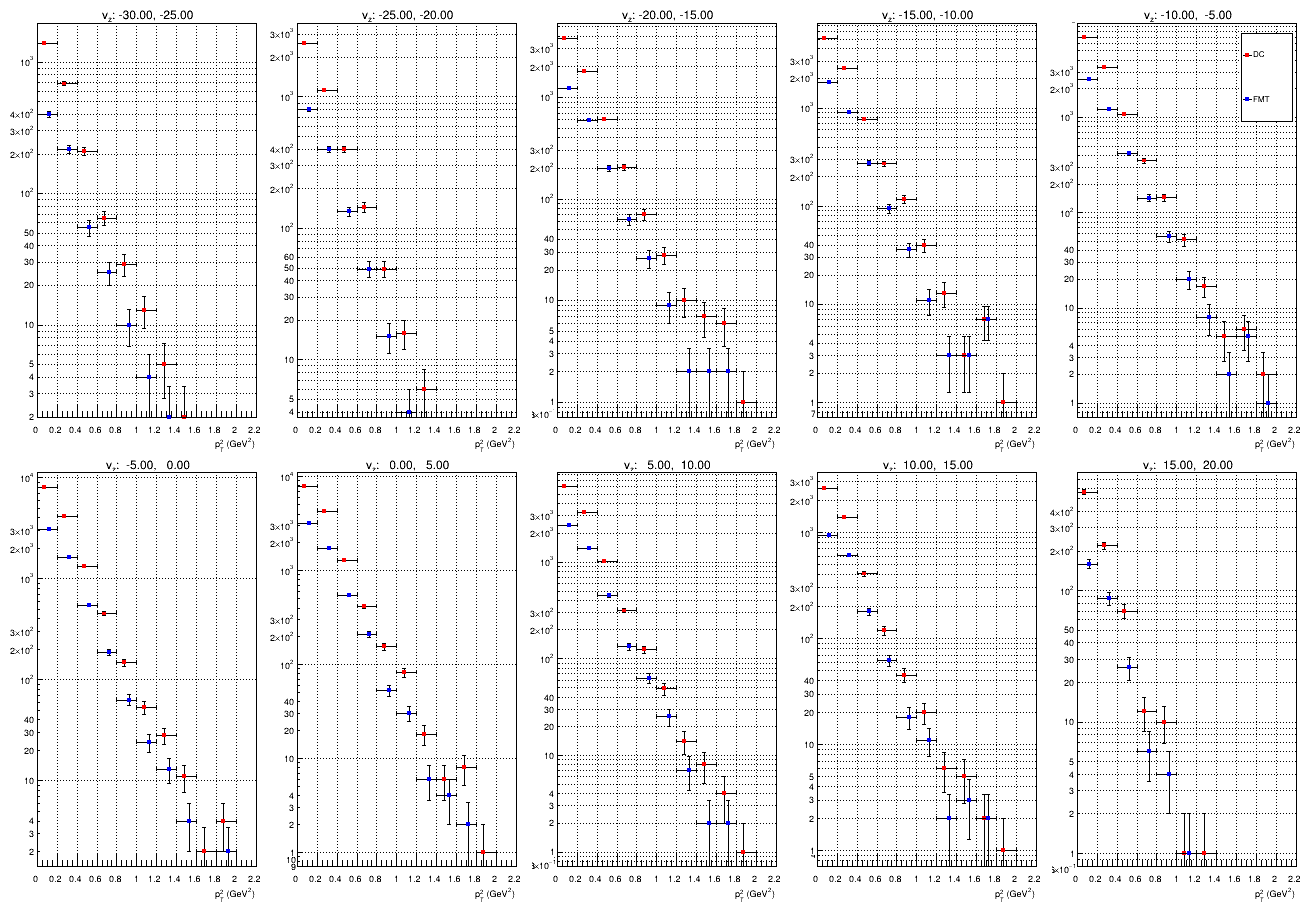
\includegraphics[width=0.72\textwidth]{10f_pt2_pi-.png}}
        }
    \end{figure}

    \backref{12.15::pt2}
\end{frame}

% --+ 20.10g phipq pi+ +--------------------------------------------------------
\begin{frame}{Uncorrected DIS Plots: $\phi_{PQ}$ for $\pi^+$}
    \label{20.10g::phipq_pi+}

    \begin{figure}[t]
        \centering{
            \fbox{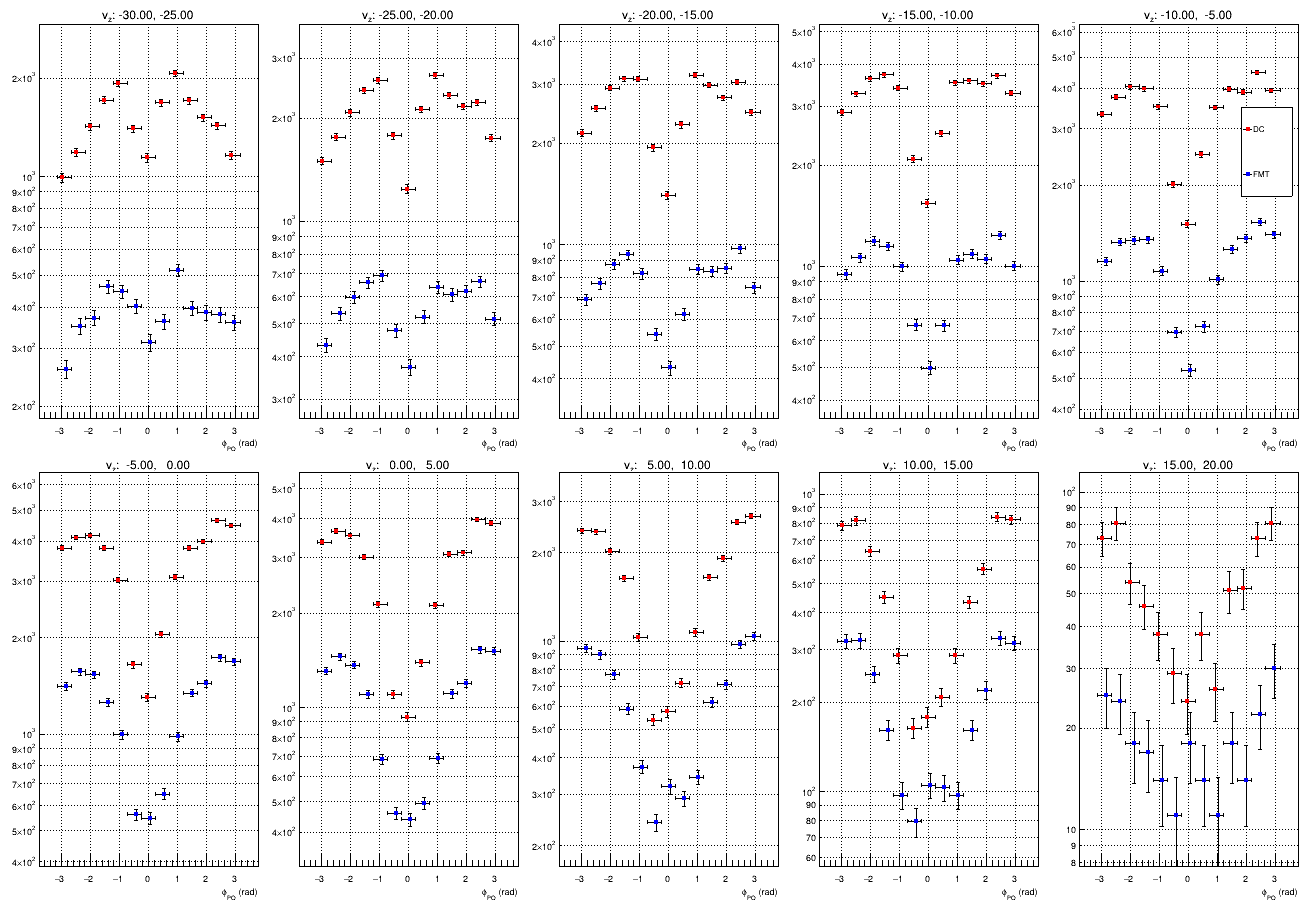
\includegraphics[width=0.72\textwidth]{10g_phipq_pi+.png}}
        }
    \end{figure}

    \backref{12.16::phipq}
\end{frame}

% --+ 20.10h phipq pi- +-----------------------------------------------------------
\begin{frame}{Uncorrected DIS Plots: $\phi_{PQ}$ for $\pi^-$}
    \label{20.10h::phipq_pi-}

    \begin{figure}[t]
        \centering{
            \fbox{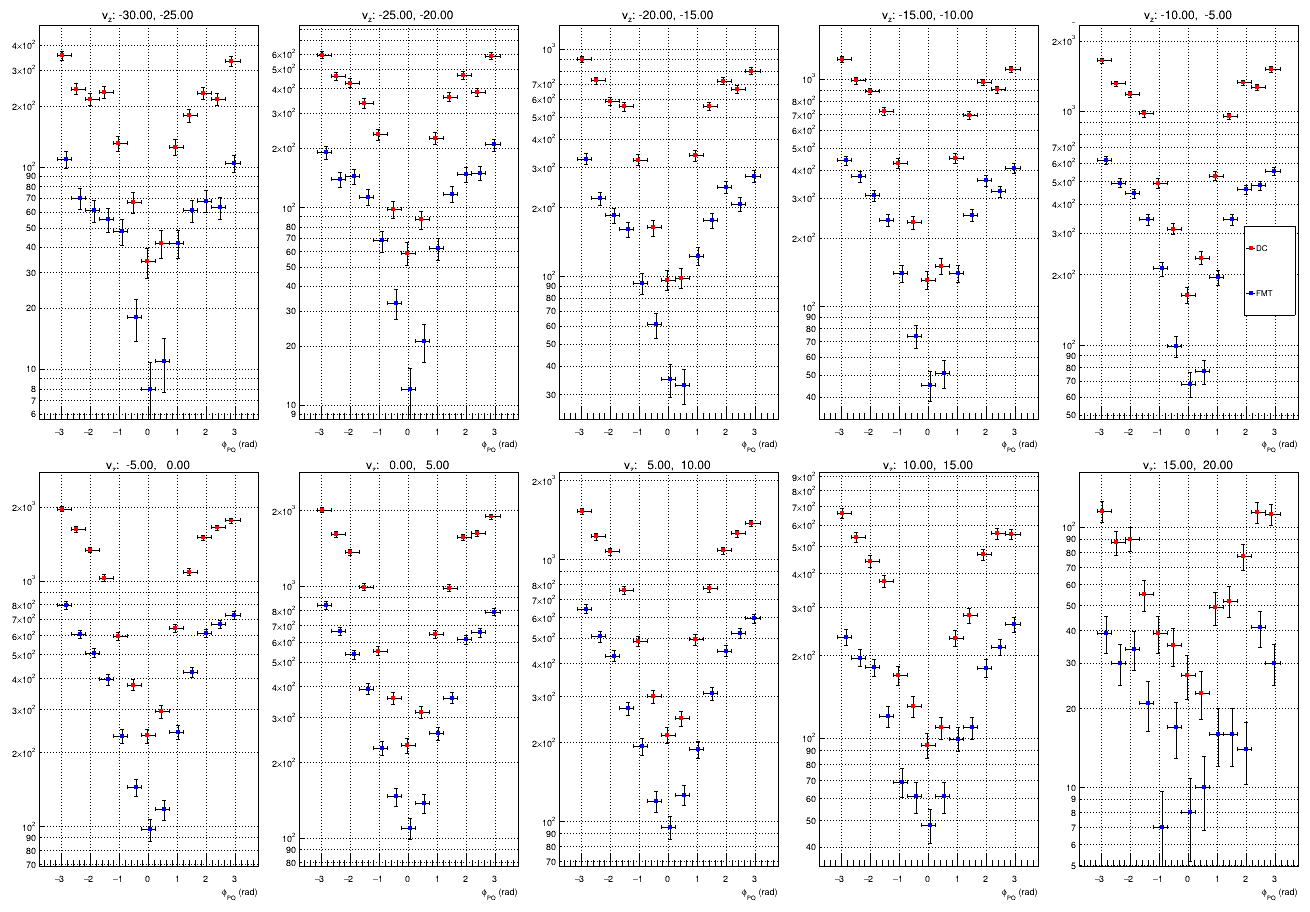
\includegraphics[width=0.72\textwidth]{10h_phipq_pi-.png}}
        }
    \end{figure}

    \backref{12.16::phipq}
\end{frame}
